% 设置 biblatex 额外选项
% \PassOptionsToPackage{gbpub=false, gbtype=false}{biblatex}

% 载入 SJTUThesis 模版
% \documentclass[degree=doctor, zihao=-4, language=english, review]{sjtuthesis}
% \documentclass[degree=master, zihao=-4]{sjtuthesis}
\documentclass[degree=bachelor, language=english, openany, oneside]{sjtuthesis}
% \documentclass[degree=course, language=english, openright, twoside]{sjtuthesis}
% 选项
%   degree=[doctor|master|bachelor|course],     % 必选,学位类型
%   language=[chinese|english],                 % 可选(默认:chinese),论文的主要语言
%   bibstyle=[gb7714-2015|gb7714-2015ay|ieee],  % 可选(默认:gb7714-2015),参考文献样式
%   review,                                     % 可选(默认:关闭),盲审模式

% 所有其它可能用到的包都统一放到这里了,可以根据自己的实际添加或者删除。
\usepackage{sjtuthesis}

% 定义图片文件目录与扩展名
\graphicspath{{figure/}}
\DeclareGraphicsExtensions{.pdf,.eps,.png,.jpg,.jpeg}

% 导入参考文献数据库
\addbibresource{bib/thesis.bib}

% 信息录入,必须在导言区进行!
% !TEX root = ../thesis.tex

%TC:ignore

\title{胆甾液晶的积分方程和密度泛函理论研究}
\author{文\quad{}聪}
\studentid{516111910163}
\supervisor{吴量}
% \assisupervisor{某某教授}
\degree{理学学士}
\major{化学(致远荣誉计划)}
\department{化学化工学院,致远学院}
\coursename{某某课程}
\date{2020年05月10日}
% \fund{国家 973 项目 (No. 2025CB000000) \\ 国家自然科学基金 (No. 81120250000)}
\keywords{液晶,统计力学,密度泛函理论}

\entitle{The Integral Equation and Density Function Theory of Cholesteric Liquids}
\enauthor{Cong Wen}
\ensupervisor{Liang Wu}
% \enassisupervisor{Prof. Uom Uom}
\endegree{Bachelor of Science}
\enmajor{Chemistry (Zhiyuan Honors Program)}
\endepartment{School of Chemistry and Chemical Engineering, Zhiyuan College}
\endate{May. 10th, 2020}
% \enfund{National Basic Research Program of China (Grant No. 2025CB000000) \\
%   National Natural Science Foundation of China (Grant No. 81120250000)}
\enkeywords{Liquid Crystal, Statistical Mechanics, Density Function Theory}

%TC:endignore


% 自定义项目标签名称
% \sjtuSetLabel{
%   listfigure = {图\quad 录},
%   listtable  = {表\quad 录}
% }

% --------------------自添命令
\newcommand{\mat}[1]{\left(\begin{matrix}#1\end{matrix}\right)}
\newcommand{\arr}[2][n]{#2_1,#2_2,\cdots,#2_{#1}}
\newcommand{\xsim}[1]{\stackrel{#1}{\sim}}
\newcommand{\iprod}[2]{\langle#1,#2\rangle}
\newcommand{\mbb}[1]{\mathbb{#1}}
\newcommand{\mbf}[1]{\mathbf{#1}}
\newcommand{\mcal}[1]{\mathcal{#1}}
\newcommand{\mfk}[1]{\mathfrak{#1}}
\newcommand{\mrm}[1]{\mathrm{#1}}
\newcommand{\mcr}[1]{\mathscr{#1}}
\newcommand{\on}[1]{\operatorname{#1}}
\newcommand{\ol}[1]{\overline{#1}}
\newcommand{\wt}[1]{\widetilde{#1}}
\newcommand{\mr}[1]{\mathring{#1}}
\newcommand{\lr}[1]{\langle{#1}\rangle}
\newcommand{\red}[1]{\textcolor{red}{#1}}
\newcommand{\blue}[1]{\textcolor{blue}{#1}}
\newcommand{\green}[1]{\textcolor{green}{#1}}
\newcommand{\tbf}[1]{\textbf{#1}}
\newcommand{\tit}[1]{\textit{#1}}
% --------------------自添命令


\begin{document}

% 无编号内容:中英文论文封面、授权页
\maketitle
\makeDeclareOriginality[pdf/originality.pdf]
\makeDeclareAuthorization

% 使用罗马数字对前言编号
\frontmatter

% 摘要
% !TEX root = ../thesis.tex

\begin{abstract}
	对于一类特殊的分子,在计算机分子模拟中观察到了其胆甾相(手性向列向),但整个计算过程仍然非常耗时,所以我们构建了一个可以更加便捷地预测这类分子热力学性质的理论框架。理论体系以Onsager的液晶相变理论为基础,以Parsons-Lee的硬球近似方法为改进,我们可以用密度泛函理论(DFT)计算出这类分子的径向分布函数(ODF)。为了预测其胆甾相,我们进一步使用Straley的近似方法,以向列相的ODF近似为胆甾相的局部ODF,从而可以预测得到液晶分子在胆甾相下的热力学性质。
\end{abstract}

\begin{enabstract}
  Cholesteric phase is found for certain liquid crystals molecules in computer simulation, but the process is still very time-consuming, so we constructed a theoretical framework to predict the thermodynamic properties of this molecule. Based on Onsager’s theory and Parsons-Lee’s improvement of phase transition of liquid crystals, we used density function theory to calculate the orientational distribution function of the molecule. And in addition, by applying Straley’s approximation method, we calculated the cholesteric pitches for a given density. We thus found a way to predict the thermodynamic properties of cholesteric liquid crystals.
\end{enabstract}


% 目录、插图目录、表格目录
\tableofcontents
\listoffigures
\listoftables
\listofalgorithms

% 主要符号、缩略词对照表
% !TEX root = ../thesis.tex

%TC:ignore

\begin{nomenclature}{rl}
\label{chap:symb}
  $\epsilon_0$ & Energy Unit \\
  $k$ & Boltzmann Constant \\
  $T$ & Temperature \\
  $\beta$ & $\frac{1}{kT}$ \\
  $O$ & Ensemble Average of a Physical Property \\
  $O^*$ & Reduced Ensemble Average of a Physical Property \\
  $F$ & Free Energy \\
  $P$ & Pressure \\
  $\mu$ & Chemical Potential \\
  $p$ & Cholesteric Pitch \\
  $q$ & $2\pi/p$, Cholesteric Pitch Wave Vector \\
  $f(\vec{u})$ & Orientational Distribution Function(ODF) \\
  $v_m$ & Molecular Volume \\
  $\rho$ & Number Density \\
  $\eta$ & $\rho v_m$, Packing Fraction\\
\end{nomenclature}

%TC:endignore


% 使用阿拉伯数字对正文编号
\mainmatter

% 论文正文
% !TEX root = ../thesis.tex

\chapter{Introduction}


This undergraduate thesis mainly investigated electrically neutral lyotropic liquid crystals, this is a kind of typical soft matter. Historically, liquid crystals were discovered in 1888 when the Australian botanist Friedrich Reinitzer studied cholesterol benzoate, which is now known as cholesteric liquid crystals, and his friend German physicist Otto Lehmann named it "Liquid Crystal".

Microscopically, liquid crystals are mostly rod-like molecules, which enables them to behave anisotropically under certain circumstances. Under high temperature (so that the kinetic energy dominates) or very low density, molecules can still move freely regardless of its rod-like shape, and they behaves just like normal fluids, this is the isotropic phase. But it can be imagined that under high density or low temperature (so that the interaction between molecules will dominate over kinetic energy), molecules are pushing each other and tend to lean on each other in a near parallel way, so they will be oriented preferably in a certain direction, this is the nematic phase. And further if they are more than rod-like, having chiral mutual interactions between each other, they further tend to lean on each other with a preferable non zero angle, behaves periodically in the space, this is the cholesteric phase.

But the understanding of liquid crystal at a molecular level is still challenging, in a preceding work by Liang\cite{Liang2017SM}, a coarse-grained molecular model is developed and represented by flexible chain with helical interactions (FCh). This is a reasonable approximation to a number of ordinary cholesteric liquid crystals, such as double strand DNA. Both nematic phase and cholesteric phase was observed by molecular dynamics (MD) simulation FCh molecules.

To further investigate how the phase transition happens and provide insight into the relationship between microscopic molecular characteristics and the macroscopic phase behavior, a theoretical method is developed in this thesis to give a prediction of thermodynamic properties of FCh model. The theory is based on Onsager's original theory\cite{Onsager1949NYAS} of phase transition of liquid crystals, and makes use of DFT method to give a depiction of the thermodynamic properties of the phase transition of FCh. In addition, a modular program is developed from scratch for the phase diagram computation of a wide range of liquid crystal molecules including FCh.


% !TeX root = ../thesis.tex
\newcommand{\mat}[1]{\left(\begin{matrix}#1\end{matrix}\right)}
\newcommand{\arr}[2][n]{#2_1,#2_2,\cdots,#2_{#1}}
\newcommand{\xsim}[1]{\stackrel{#1}{\sim}}
\newcommand{\iprod}[2]{\langle#1,#2\rangle}
\newcommand{\mbb}[1]{\mathbb{#1}}
\newcommand{\mbf}[1]{\mathbf{#1}}
\newcommand{\mcal}[1]{\mathcal{#1}}
\newcommand{\mfk}[1]{\mathfrak{#1}}
\newcommand{\mrm}[1]{\mathrm{#1}}
\newcommand{\mcr}[1]{\mathscr{#1}}
\newcommand{\on}[1]{\operatorname{#1}}
\newcommand{\ol}[1]{\overline{#1}}
\newcommand{\wt}[1]{\widetilde{#1}}
\newcommand{\mr}[1]{\mathring{#1}}
\newcommand{\lr}[1]{\langle{#1}\rangle}
\newcommand{\red}[1]{\textcolor{red}{#1}}
\newcommand{\blue}[1]{\textcolor{blue}{#1}}
\newcommand{\green}[1]{\textcolor{green}{#1}}
\newcommand{\tbf}[1]{\textbf{#1}}
\newcommand{\tit}[1]{\textit{#1}}

\chapter{Theoretical Framework}

\section{Statistical Mechanics}
\subsection{Theory of Ensembles}

\subsection{Liquid Crystal Theory of Onsager}

\subsection{Parsons-Lee's Approximation}

\subsection{Straley's Method}

\section{Density Function Theory}
\subsection{Variation Method}

\subsection{Iteration Equation}

\section{Application to FCh Model}
This section collects the concrete computation of properties of FCh model.


First, write
\begin{equation}
	F^*=F_{id}^*+F_{ex}^*,
\end{equation}
the first term is
\begin{equation}
	F_{id}^*=\ln\eta-1+\int\on{d}\vec{u}f(\vec{u})\ln f(\vec{u}),
\end{equation}
then due to Straley[], we have
\begin{align}
	F_{ex}^*&=\frac{\eta}{2}\int\on{d}\vec{u}_1\on{d}\vec{u}_2M_0^*(\vec{u}_1,\vec{u}_2)f(\vec{u}_1)f(\vec{u}_2)-K_t^*q+\frac{1}{2}K_2^*q^2\\
	K_t^*&=-\frac{\eta}{2}\int\on{d}\vec{u}_1\on{d}\vec{u}_2M_1^*(\vec{u}_1,\vec{u}_2)f(\vec{u}_1)f'(\vec{u}_2)u_{2y}\\
	K_2^*&=-\frac{\eta}{2}\int\on{d}\vec{u}_1\on{d}\vec{u}_2M_2^*(\vec{u}_1,\vec{u}_2)f'(\vec{u}_1)f'(\vec{u}_2)u_{1y}u_{2y}\\
\end{align}
and in which the reduced $k$-th moment is given by
\begin{equation}
	M_k^*(\vec{u}_1,\vec{u}_2)=\frac{1}{v_m}\int\on{d}\vec{r}_c\left[e^{-\beta U(\vec{r}_c,\vec{u}_1,\vec{u}_2)}-1\right]r_{cz}^k
\end{equation}

In addition, the first term of $F_ex^*$ is divided into two parts(due to Parsons-Lee)
\begin{equation}
	\begin{split}
	\frac{\eta}{2}\int\on{d}\vec{u}_1\on{d}\vec{u}_2M_0^*(\vec{u}_1,\vec{u}_2)f(\vec{u}_1)f(\vec{u}_2)&=G(\eta)V_{int}\\
	&+\frac{\eta}{2}A_{int}
	\end{split}
\end{equation}

in which $G(\eta)=\dfrac{4\eta-3\eta^2}{8(1-\eta)^2}$, and
\begin{align}
V^*(\vec{u}_1,\vec{u}_2)=\frac{1}{v_m}\int\on{d}\vec{r}_c\left[e^{-\beta U_{rep}(\vec{r}_c,\vec{u}_1,\vec{u}_2)}-1\right],\\
V_{int} = \int\on{d}\vec{u}_1\on{d}\vec{u}_2V^*(\vec{u}_1,\vec{u}_2)f(\vec{u}_1)f(\vec{u}_2), \\
A^*(\vec{u}_1,\vec{u}_2)=\frac{1}{v_m}\int\on{d}\vec{r}_c\left[e^{-\beta U_{att}(\vec{r}_c,\vec{u}_1,\vec{u}_2)}-1\right],\\
A_{int}=\int\on{d}\vec{u}_1\on{d}\vec{u}_2A^*(\vec{u}_1,\vec{u}_2)f(\vec{u}_1)f(\vec{u}_2).
\end{align}

Up to now all the required quantities are presented. In the next section we write down explicitly all the important physical properties.

\section{Properties}
\subsection{Reduced free energy}
\begin{equation}
	\begin{split}
	F^*&=\ln\eta -1+\int\on{d}\vec{u}f(\vec{u})\ln f(\vec{u})+\frac{4\eta-3\eta^2}{8(1-\eta)^2}V_{int}+\frac{\eta}{2}A_{int}-K_t^*q+\frac{1}{2}K_2^*q^2
	\end{split}
\end{equation}

\subsection{Reduced Pressure}
The reduced pressure $P^*=\beta v_m P=\eta^2\dfrac{\partial F^*}{\partial\eta}$
\begin{equation}
	P^* = \eta + \frac{\eta^2(2-\eta)}{4(1-\eta)^3}V_{int}+\frac{1}{2}\eta^2A_{int}-\frac{1}{2}\eta K_t^*q
\end{equation}

\subsection{Chemical Potential}
The reduced chemical potential $\mu^*=\beta\mu=\eta\dfrac{\partial F^*}{\partial\eta}+F^*$
\begin{equation}
	\mu^*=\ln\eta+\int\on{d}\vec{u}f(\vec{u})\ln f(\vec{u})+\frac{\eta(3\eta^2-9\eta+8)}{8(1-\eta)^3}V_{int}+\eta A_{int}-K_t^*q
\end{equation}

\section{DFT part}
This part deals with the calculation of ODF by minimizing the free energy without cholesteric terms, i.e. in the pure nematic phase
\begin{equation}
	F_{n}^*=\ln\eta -1+\int\on{d}\vec{u}f(\vec{u})\ln f(\vec{u})+G(\eta)V_{int}+\frac{\eta}{2}A_{int}
\end{equation}
Now we need to minimize the above expression with respect to $\int f(\vec{u})\on{d}\vec{u}=1$, so consider the variation with respect to $f$, for convenience, take $f_{\epsilon}=f+\epsilon g$ then we require
\begin{equation}
	\frac{\partial}{\partial\epsilon}\left[F_{n}^*(f_{\epsilon})+\lambda\left(\int f_{\epsilon}\on{d}\vec{u}-1\right)\right]|_{\epsilon=0}=0, \forall g
\end{equation}
By calculation, this gives
\begin{equation}
	\int\on{d}\vec{u}_1g(\vec{u}_1)\left(1+\ln f(\vec{u}_1)+2G(\eta)\int\on{d}\vec{u}_2f(\vec{u}_2)V^*(\vec{u}_1,\vec{u}_2))+\eta\int\on{d}\vec{u}_2f(\vec{u}_2)A^*(\vec{u}_1,\vec{u}_2))+\lambda\right)=0
\end{equation}
Hence
\begin{equation}
	1+\lambda+\ln f(\vec{u}_1)+2G(\eta)\int\on{d}\vec{u}_2f(\vec{u}_2)V^*(\vec{u}_1,\vec{u}_2))+\eta\int\on{d}\vec{u}_2f(\vec{u}_2)A^*(\vec{u}_1,\vec{u}_2))=0
\end{equation}
By writing
\begin{equation}
	\begin{split}
		I^{rep}(\vec{u})&=2G(\eta)\int\on{d}\vec{u}_2f(\vec{u}_2)V^*(\vec{u},\vec{u}_2)\\
		I^{att}(\vec{u})&=\eta\int\on{d}\vec{u}_2f(\vec{u}_2)A^*(\vec{u},\vec{u}_2))
	\end{split}
\end{equation}

The iteration equation is given by
\begin{equation}
	f_{n+1}(\vec{u})=\on{Norm}\left(e^{-I_n^{rep}(\vec{u})-I_n^{att}(\vec{u})}\right)
\end{equation}
in which $\on{Norm}$ means normalizing the integral over all $\vec{u}$ to $1$.


% !TeX root = ../thesis.tex

\chapter{Application to FCh model}\label{chap:model}

\section{Flexible Chain with Helical Interactions (FCh)}
The molecular model is given in Fig. \ref{fig:fch},
\begin{figure}[H]
 	\centering
 	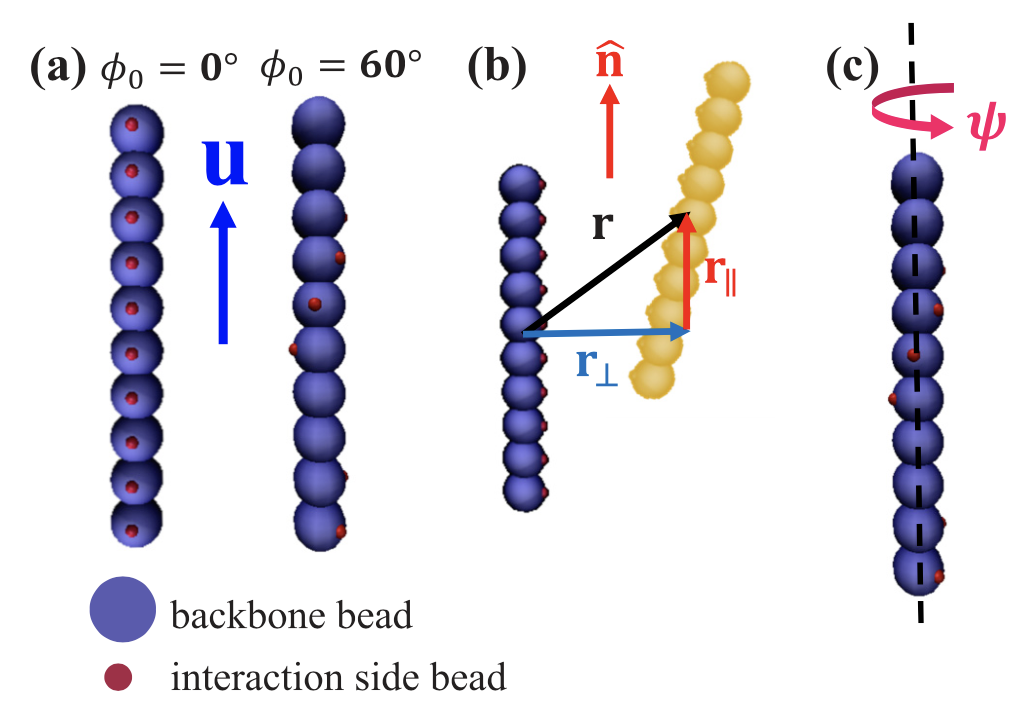
\includegraphics[width=\linewidth]{fch.png}
	\caption[Schematic of FCh model]{Schematic figure of FCh model\cite{Liang2019PRE}}
	\label{fig:fch}
\end{figure}

There are several defining parameters of a FCh molecule $(m,\phi_0)$, the former is the length of FCh and the latter is its helix internal angle. In addition, to identify a FCh molecule in the space, it suffices to use $(q,u,\phi)$, in which $q$ is the position of center of mass, $u$ is the orientation, and $\phi$ is the internal azimuthal angle.

Denote by $\sigma$ the length unit, $\epsilon$ the energy unit, $\sigma_b = 2^{1/6}\sigma$ and $\sigma_i = 0.1\sigma_b$ are the diameter of the backbone bead and interaction site bead. And there are two kinds of interactions involved, soft repulsion between backbone beads by Weeks-Chandler-Anderson (WCA) potential, short-ranged attractions between interaction beads by shifted Lennard-Jones (sLJ) potential truncated at $r_c=2.5\sigma$.

\begin{equation}
	U_{\mathrm{WCA}}(r)=\left\{
	\begin{array}{ll}
		4 \epsilon\left[\left(\frac{\sigma_b}{r}\right)^{12}-\left(\frac{\sigma_b}{r}\right)^{6}\right]+\epsilon & r<\sigma_b \\ 0 & r \geq \sigma_b
	\end{array}\right.
\end{equation}

\begin{equation}
	U_{\mathrm{sLJ}}(r)=\left\{
	\begin{array}{ll}
		4 \epsilon\left[\left(\frac{\sigma_i}{r}\right)^{12}-\left(\frac{\sigma_i}{r}\right)^{6}\right]-U_{\mathrm{LJ}}\left(r_c\right) & r<2.5 \sigma\\0 & r \geq 2.5 \sigma
	\end{array}\right.
\end{equation}

As for the potential between backbone and interaction beads, it is sLJ potential with parameters are derived by Lorentz-Berthelot mixing rule in the previous simulation work, but here it is ignored, there only b-b interaction and i-i interaction in this theoretical work.

\section{Existing Simulation Results}\label{Sec:SimRes}
Molecular dynamics simulations were performed in the paper and it is found there are three existing phases, isotopic, nematic and cholesteric. To illustrate further, take the example in case of $m=10, \phi_0=30^\circ$, the pressure and phase diagram is shown below.

\begin{figure}[H]
 	\centering
 	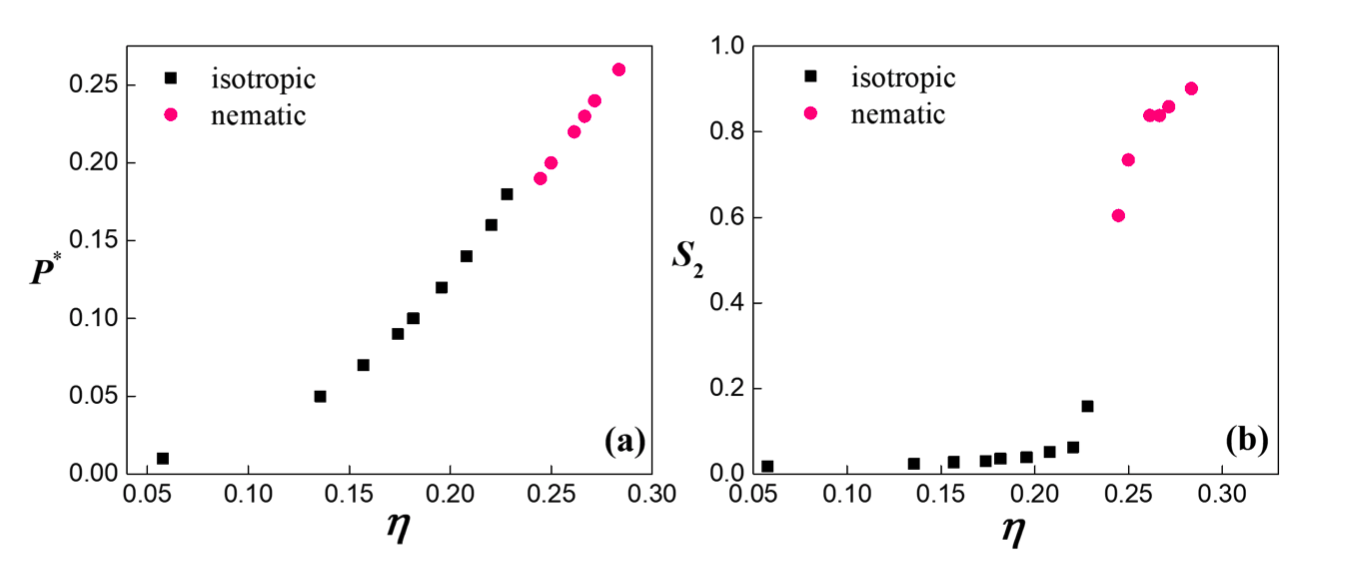
\includegraphics[width=\linewidth]{phaseDiag.png}
	\caption[Phase diagram of FCh using MD simulation]{Phase Diagram of FCh using MD simulation\cite{Liang2019PRE}}
	\label{fig:MDdiag}
\end{figure}

Note in the diagram, $P^*=P\sigma^3/\epsilon$. And in this figure we know the transition pressure and transition packing fraction are $P_0^*=0.1v_m=1.332, \eta_0=0.24$

\section{DFT of FCh Model}
This part will make use of all the methods introduced before and apply to FCh model. In particular, we will illustrate how to use variational method and iteration to find out ODF which corresponds to the minimal free energy.

Recall that the free energy is unpacked into two parts,
\begin{equation}
	F^*=F_{id}^*+F_{ex}^*,
\end{equation}
the first term contains both free energy of ideal gas and the entropy contributed by ODF,
\begin{equation}
	F_{id}^*=\ln\eta-1+\int\on{d}uf(u)\ln f(u),
\end{equation}
in fact the first term is $\ln\rho\Lambda^3$, but this does not matter because it only differs by a constant with $\ln\eta$.

Then due to Straley\cite{Straley1973Frank, Straley1976Theory} , the excess free energy is written in the form
\begin{align}
	F_{ex}^*&=\frac{\eta}{2}\int\on{d}u_1\on{d}u_2M_0^*(u_1,u_2)\varphi(u_1)\varphi(u_2)-K_t^*q+\frac{1}{2}K_2^*q^2\\
	K_t^*&=-\frac{\eta}{2}\int\on{d}u_1\on{d}u_2M_1^*(u_1,u_2)\varphi(u_1)\varphi'(u_2)u_{2y}\\
	K_2^*&=-\frac{\eta}{2}\int\on{d}u_1\on{d}u_2M_2^*(u_1,u_2)\varphi'(u_1)\varphi'(u_2)u_{1y}u_{2y}
\end{align}
and in which $M_k$ has been defined above.

In addition, the first term of $F_{ex}^*$ can be further divided into repulsion part and attractive part, the repulsion part can then be approximated by Parsons-Lee's method,
\begin{equation}
	\frac{\eta}{2}\int\on{d}u_1\on{d}u_2M_0^*(u_1,u_2)\varphi(u_1)\varphi(u_2)=G(\eta)V_{int}+\frac{\eta}{2}A_{int}.
\end{equation}

in which $V_{int}$ and $A_{int}$ is the abbreviation for two integrals, they will be used further in the calculation of other physical properties,
\begin{equation}\label{Eqn:VAstar}
	\begin{split}
		V^*(u_1,u_2)=\frac{1}{v_m}\int\on{d}q\left[1-e^{-\beta U_{rep}(0,u_1;q,u_2)}\right],\\
		V_{int} = \int\on{d}u_1\on{d}u_2V^*(u_1,u_2)\varphi(u_1)\varphi(u_2), \\
		A^*(u_1,u_2)=\frac{1}{v_m}\int\on{d}q\left[1-e^{-\beta U_{att}(0,u_1;q,u_2)}\right],\\
		A_{int}=\int\on{d}u_1\on{d}u_2A^*(u_1,u_2)\varphi(u_1)\varphi(u_2).
	\end{split}
\end{equation}

According to Sec. \ref{Sec:Joachim}, the expression for $V^*$ can be approximated directly by Eqn. \ref{Eqn:Joachim}, since the repulsion interaction in FCh model is nearly hard.

Up to now all the required quantities are presented. In the next section we write down explicitly all the important physical properties.

\section{Properties}
All the properties calculated in this part should be calculated after computing ODF using iteration method, but for logical coherence, we derive them first.

Remark: keep in mind that $F^*\equiv\beta F/N$.
\subsection{Reduced free energy}
The general expression of reduced free energy can be collected into one expression
\begin{equation}\label{Eqn:FreeEne}
	F^*=\ln\eta -1+\int\on{d}u\varphi(u)\ln \varphi(u)+\frac{4\eta-3\eta^2}{8(1-\eta)^2}V_{int}+\frac{\eta}{2}A_{int}-K_t^*q+\frac{1}{2}K_2^*q^2.
\end{equation}
To be more precise, the expression above is the free energy of cholesteric phase, as for the free energy of nematic phase, the last two terms are dropped
\begin{equation}\label{Eqn:EneNem}
	F_{n}^*=\ln\eta -1+\int\on{d}u\varphi(u)\ln \varphi(u)+\frac{4\eta-3\eta^2}{8(1-\eta)^2}V_{int}+\frac{\eta}{2}A_{int}.
\end{equation}
And as for the free energy of isotropic phase, it suffices to let $\varphi(u)\equiv \frac{1}{4\pi}$ and substitute into Eqn. \ref{Eqn:EneNem}.

\subsection{Reduced Pressure}
The reduced pressure $P^*=\beta v_m P=-\beta v_m \dfrac{\partial F}{\partial V}= \eta^2\dfrac{\partial F^*}{\partial\eta}$
\begin{equation}\label{Eqn:Press}
	P^* = \eta + \frac{\eta^2(2-\eta)}{4(1-\eta)^3}V_{int}+\frac{1}{2}\eta^2A_{int}-\frac{1}{2}\eta K_t^*q
\end{equation}

\subsection{Chemical Potential}
The reduced chemical potential $\mu^*=\beta\mu=\beta\dfrac{\partial F}{\partial N}=\eta\dfrac{\partial F^*}{\partial\eta}+F^*$
\begin{equation}\label{Eqn:ChemPot}
	\mu^*=\ln\eta+\int\on{d}u\varphi(u)\ln \varphi(u)+\frac{\eta(3\eta^2-9\eta+8)}{8(1-\eta)^3}V_{int}+\eta A_{int}-K_t^*q.
\end{equation}

\subsection{Order Parameter}
The order parameter is standard from Onsager's theory
\begin{equation}
	S_2=\int \on{d}u\varphi(u)\left[\frac{1}{2}(3\cos^2\theta -1)\right],
\end{equation}
in which $\theta$ is the angle between $u$ and $e_3$, precisely given by $\cos\theta = u_z = u\cdot e_3$.

\section{Code Calibration: Hard Spherocylinders (HSC) Model}
To verify the correctness of the computation program, we used the data from Jackson's work\cite{Jackson1996JCP} in 1996. In the paper the author re-examined the phase diagram of hard spherocylinders by Monte-Carlo simulation in a canonical ensemble. The schematic of hard spherocylinders is given below. We used our theoretical method to calculate the phase diagram of HSC, and the result is in well accordance with Jackson's simulation results.

\begin{figure}[H]
 	\centering
 	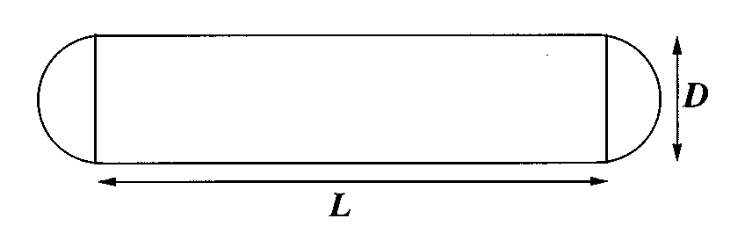
\includegraphics[width=\linewidth]{HSC.png}
	\caption[Schematic of Hard Spherocylinders]{Schematic of Hard Spherocylinders\cite{Jackson1996JCP}}
	\label{fig:MDdiag}
\end{figure}

Jackson et al. calculated HSC with four different ratio of length and diameter $\kappa=L/D=3,3.2,4,5$, and the nematic-isotropic transition point is compared in the next table.

\begin{table}[H]
	\caption{Comparison of transition point}
	\label{tab:comparison1995}
	\centering
	\begin{tabular}{c|cccc}
		\toprule
		 & $\kappa=3$ & $\kappa=3.2$ & $\kappa=4$ & $\kappa=5$\\
		\midrule
		$\eta_{MC}$ &  $0.577$ & $0.513$ & $0.472$ & $0.408$\\
		$\eta_{DFT}$ & $0.530$ & $0.515$ & $0.460$ & $0.405$\\
		\bottomrule
	\end{tabular}
\end{table}

It can be seen from Tab. \ref{tab:comparison1995} that the result given by DFT method is in accordance with the result given by Monte Carlo method in a canonical ensemble. The more detailed data of pressure is also in well accordance.


\section{Program Development}
To calculate all the properties and phase diagram mentioned above, a whole program in C++ has been implemented from scratch and been uploaded on \href{https://github.com/WolframC/liquidcrystal}{Github}. The program is transferrable for different kind of liquid crystals as long as the class which defined the molecule structure is added.

Overall, the program contains three main features
\begin{enumerate}
	\item Monte Carlo computation of ensemble average of quantities in terms of energy.
	\item Computation of ODF by iteration method.
	\item Calculation of free energy and remaining physical properties.
\end{enumerate}

And this section serve as both a report for what has been done and instructions for those who need to continue the liquid crystal project study. We first recapitulate the expressions we are going to compute, and further in following chapters we illustrate concrete implementation involved.

\subsection{Monte Carlo Method}
According to the theory introduced before, we need to first calculate properties which are irrelevant to ODF, namely, they are $A^*, V^*, M_k^*$ (which are given by Eqn. \ref{Eqn:VAstar}, Eqn. \ref{Eqn:Mk}). To see how they are calculated, $V^*$ has been given by Joachim's approximation in Eqn. \ref{Eqn:Joachim}. And $A^*, M_k^*$ are computed using Monte Carlo method.
\begin{equation*}	
	\begin{split}
		V^*(u_1,u_2)=11-\frac{3}{m}&+3.5339(m+\frac{1}{m}-2)\sin\theta,  \cos\theta=u_1\cdot u_2,\\
		A^*(u_1,u_2)&=\frac{1}{v_m}\int\on{d}q\left[1-e^{-\beta U_{att}(0,u_1;q,u_2)}\right],\\
		M_k^*(u_1,u_2)&=\frac{1}{v_m}\int\on{d}q \left[1-e^{-\beta u(0,u_1;q,u_2)}\right]q_z^k.
	\end{split}
\end{equation*}

Note that in fact to identify a FCh model, it is necessary to designate at least three parameters: $(q,u,\phi)$, in which $q$ denotes the coordinate of its center of mass, $u$ denotes its orientation, and $\phi$ denotes the internal azimuthal angle. So the integral in $A^*,M_k^*$ has to be slightly modified and made more precise:

\begin{equation}
	\begin{split}
		A^*(u_1,u_2)&=\frac{1}{v_m}\int_V\on{d}q \int_0^{2\pi}\on{d}\phi_1\int_0^{2\pi}\on{d}\phi_2 \left[1-e^{-\beta U_{att}(0,u_1,\phi_1;q,u_2,\phi_2)}\right],\\
		M_k^*(u_1,u_2)&=\frac{1}{v_m}\int_V\on{d}q \int_0^{2\pi}\on{d}\phi_1\int_0^{2\pi}\on{d}\phi_2 \left[1-e^{-\beta u(0,u_1, \phi_1; q,u_2, \phi_2)}\right]q_z^k.
	\end{split}
\end{equation}

In the expression $V$ is taken to be the whole space in which MC process will take place, and let the length scale on one dimension to be two times of a single molecule, i.e. denote $L = 2m\sigma_b$.

Since the two integrals are of the same type, we only illustrate the computation for $M_k^*$. By using cylindrical coordinates, write $\on{d}q=r\on{d}r\on{d}z\on{d}\phi$. Then the expression of $M_k^*$ becomes
\begin{equation}\label{Eqn:IntegMk}
	M_k^*(u_1,u_2)=\frac{2\pi}{v_m}\int_{-L/2}^{L/2}\on{d}z\int_{-L/2}^{L/2}\on{d}r \int_0^{2\pi}\on{d}\phi_1\int_0^{2\pi}\on{d}\phi_2 \left[1-e^{-\beta u(0,u_1, \phi_1; q,u_2, \phi_2)}\right]z^kr.
\end{equation}

Except for using Monte Carlo method to estimate the preceding integral, we can also use an averaged method by dividing $z,r,\phi_1,\phi_2$ into uniform pieces. In practice, $z,r$ are always taken to be divided into $50$ pieces and $\phi_1,\phi_2$ are divided into $10$ pieces.

\subsubsection{Collision Detection}
In the estimation of the integral introduced above, there are many pairs of configurations which made $u(0,u_1,\phi_1;q,u_2,\phi_2)=0$ and hence contributes nothing to the whole integral, since the interaction between FCh molecules are relatively short-ranged. So we can calculate the shortest distance between two molecules and judge if it is within the cutoff distance to optimize the integral computation. We give the algorithm here without proof, since it is easy with elementary vector analysis.

\begin{algorithm}[H]
	\caption{Shortest Distance between a Point and a Segment}
	\label{Alg:DisPointSeg}
	\KwData{point $\vec{p}$, start point of the segment $\vec{s}$, end point of the segment $\vec{t}$}
	\KwResult{shortest distance $d$ between $\vec{p}$ and the segment defined by $\vec{s},\vec{t}$}
	$\vec{u}\leftarrow\dfrac{\vec{t}-\vec{s}}{\|\vec{t}-\vec{s}\|_2}$\;
	$\vec{ps}\leftarrow\vec{p}-\vec{s}$, $\vec{pt}\leftarrow\vec{p}-\vec{t}$\;
	\uIf{$\vec{u}\cdot\vec{ps}<0$}{
		$d\leftarrow\|\vec{ps}\|_2$\;
	}\uElseIf{$\vec{u}\cdot\vec{pt}>0$}{
		$d\leftarrow\|\vec{pt}\|_2$\;
	}\Else{
		$d\leftarrow\|\vec{u}\times\vec{ps}\|_2$\;
	}
\end{algorithm}

\begin{algorithm}[H]
	\caption{Shortest Distance between Two Segments}
	\label{Alg:DisSegSeg}
	\KwData{length, center and unit orientation vector of the segment $l_i, \vec{r}_i, \vec{u}_i$}
	\KwResult{shortest distance $d$ between the two segment}
	$\vec{s}\leftarrow\vec{r}_1-\vec{r}_2$\;
	$f\leftarrow$True\;
	\uIf{$1-(\vec{u}_1\cdot\vec{u}_2)^2=0$}{
		$f\leftarrow$False\tcp*[l]{Parallel segments}
	}\Else{
		$\lambda_1\leftarrow\dfrac{1}{1-(\vec{u}_1\cdot\vec{u}_2)^2}\left(-\vec{s}\cdot\vec{u}_1+(\vec{s}\cdot\vec{u}_2)(\vec{u}_1\cdot\vec{u}_2)\right)$\;
		$\lambda_2\leftarrow\dfrac{1}{1-(\vec{u}_1\cdot\vec{u}_2)^2}\left(\vec{s}\cdot\vec{u}_2-(\vec{s}\cdot\vec{u}_1)(\vec{u}_1\cdot\vec{u}_2)\right)$\;
		
		\eIf{$\left(|\lambda_1| > l_1/2\right) \vee \left(|\lambda_2|>l_2/2\right)$}{
			$f\leftarrow$False\tcp*[l]{Skew segments}
		}{
			$f\leftarrow$True\tcp*[l]{Segments intesects}
		}
	}
	
	\eIf{$f$}{
		$d\leftarrow\|\vec{s}+\lambda_1\vec{u}_1-\lambda_2\vec{u}_2\|_2$
	}{
		$d$ is taken to be the minimum of four shortest distance from four endpoints to the other segments using Alg. \ref{Alg:DisPointSeg}.
	}
\end{algorithm}

Using the algorithms introduced above, the efficiency of Monte Carlo estimation of the integral can be largely improved.

\subsection{DFT calculation}
With all the data coming from the Monte Carlo method, using iteration to find out the corresponding ODF with a given packing fraction $\eta$ can be directly performed, which has been already illustrated in Sec. \ref{Sec:Iter}. But to clarify here, we must point out the concrete discretization method of a function on the sphere. we divide every longitude line into $20$ parts, and latitude line into $40$ part (except at two poles), so this gives $40\times 19+2 = 762$ point on the sphere. Hence the ODF is actually a $762$-dimensional vector in computation code. So $\on{d}\phi=\on{d}\theta =\pi/20$And $\on{d}u$ actually becomes $\dfrac{\pi^2}{400}\sin\phi$, with $u\cdot e_3=\cos\phi$.

\section{Iteration Process}

The DFT process should give a convergent result of ODF, we put an example here showing this.
\begin{figure}[H]
 	\centering
 	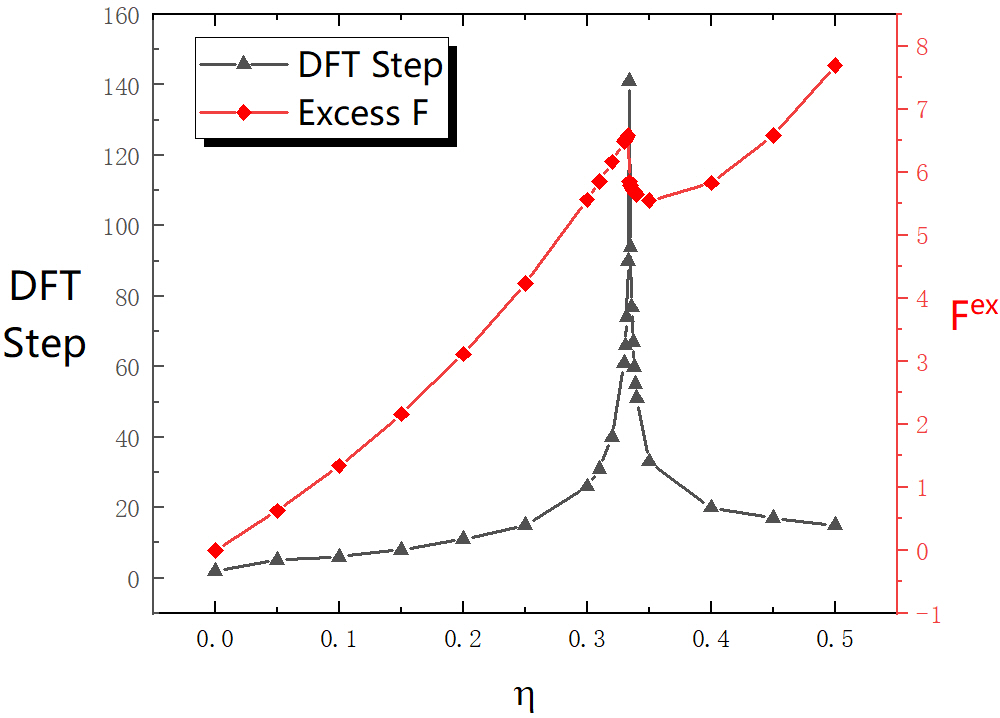
\includegraphics[width=0.8\linewidth]{snf.jpg} \\
	\caption[Step of DFT process]{Step of DFT process}
	\label{fig:DFTstep}
\end{figure}
From this we can see that near the first-order transition point, the iteration step reaches a peak, which means it the state is very non stable near transition and may jump between two different states.

\section{The Isotropic-Nematic Phase Transition}
The isotropic-Nematic phase transition is observed using this theoretical method, and a typical result of physical properties at $m=10, \phi_0=30^\circ$ is given below. A sudden change in the order parameter implies an isotropic-nematic phase transition, and we can also see that the free energy of nematic phase is lower than free energy of isotropic phase.
\begin{figure}[H]
	\begin{minipage}{0.5\textwidth}
		\centering
		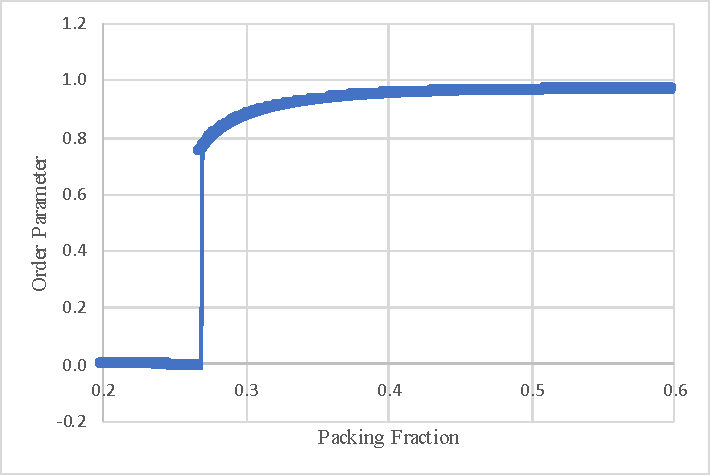
\includegraphics[width=\linewidth]{orderparam.pdf}
		\caption{Relation between order parameter and packing fraction}
		\label{fig:orderParam}
	\end{minipage}\hfill
	\begin{minipage}{0.5\textwidth}
 		\centering
 		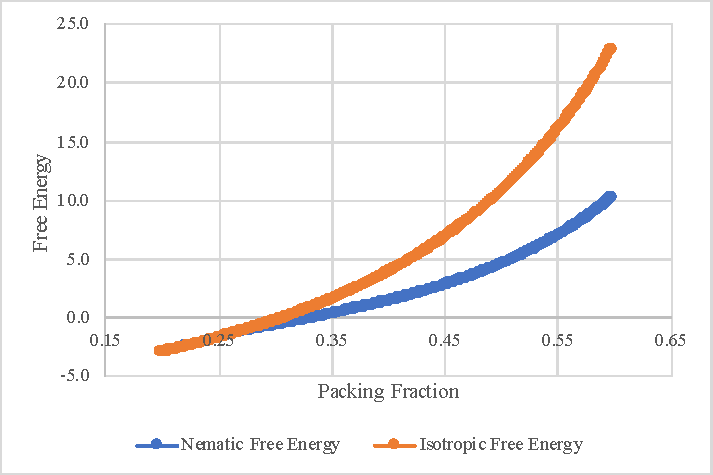
\includegraphics[width=\linewidth]{freeEne.pdf}
 		\caption{Free energy of isotropic and nematic phases}
 		\label{fig:freeEne}
 	\end{minipage}
\end{figure}

And the sudden change at $\eta=0.268$ can also be seen in the diagram of pressure and chemical potential, there is a sudden decline as well as the case in free energy. This is the typical characteristic of a first-order transition.
\begin{figure}[H]
	\begin{minipage}{0.5\textwidth}
		\centering
		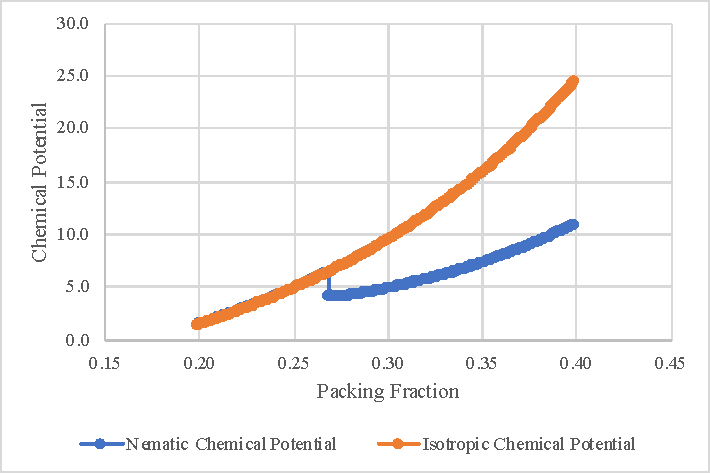
\includegraphics[width=\linewidth]{1030chemPot.pdf}
		\caption{Chemical potential of isotropic and nematic phase}
		\label{fig:chemPot}
	\end{minipage}\hfill
	\begin{minipage}{0.5\textwidth}
 		\centering
 		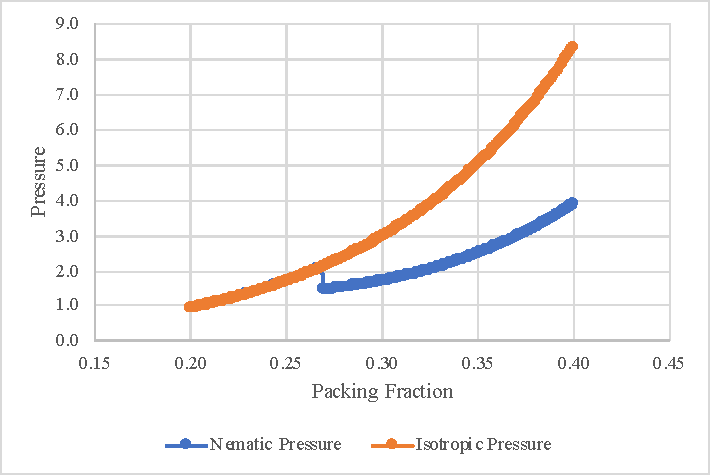
\includegraphics[width=\linewidth]{1030press.pdf}
 		\caption{Pressure of isotropic and nematic phase}
 		\label{fig:press}
 	\end{minipage}
\end{figure}

In addition, we compared the transition point at different length and internal azimuthal angle, the following are the data of transition point for FCh model of length $m=10,15,20$ and internal azimuthal angle $\phi_0=15^\circ, 30^\circ, 45^\circ, 60^\circ$.

\begin{figure}[H]
 	\centering
 	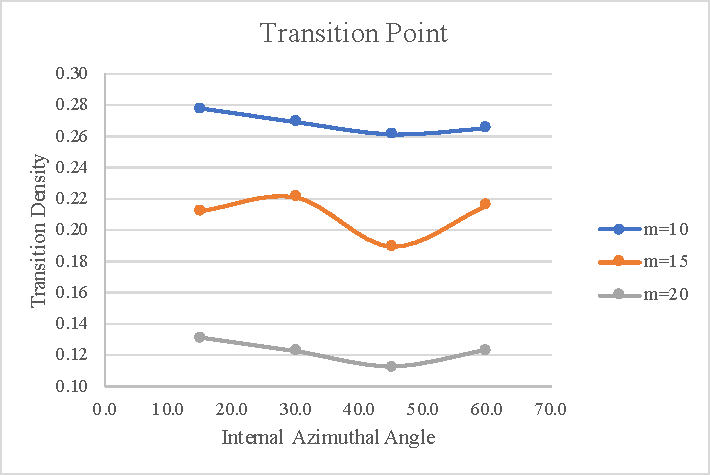
\includegraphics[width=0.8\linewidth]{transition.pdf} \\
	\caption[Schematic of coordinates]{Transition point of FCh}
	\label{fig:tran}
\end{figure}

It can be seen from the figure that $45^\circ$ might be a preferred internal azimuthal angle at which two adjacent FCh molecules have the strongest mutual interaction, making it more easily to undergo phase transition. As for a given internal azimuthal angel, the longer the molecule is, the larger its orientational entropy contributes to the free energy, since phase transition is in fact a balance between energy and entropy, the larger contribution from orientational entropy will result in smaller packing fraction.

\section{The Cholesteric Pitch}
The calculation for cholesteric pitch is still not clear since the computation of $K_t^*$ always gives a zero. It is very important here to note when doing integration for $M_k^*$, we need to make sure that $M_1(u_1,u_2)\neq M_1(u_2,u_1)$, otherwise $K_t^*$ must be zero. This can be seen from the following derivation by writing $\on{d}u=\sin\phi\on{d}\phi\on{d}\theta$
\begin{equation}
	\begin{split}
		K_t^*&=-\frac{\eta}{2}\int\on{d}u_1\on{d}u_2M_1^*(u_1,u_2)\varphi(u_1)\varphi'(u_2)u_{2y}\\
		&=-\frac{\eta}{2}\int_{-\pi/2}^{\pi/2}\on{d}\phi_1\varphi(\phi_1)\sin\phi_1\int_{-\pi/2}^{\pi/2}\on{d}\phi_2\varphi'(\phi_2)\sin^2\phi_2\int_{-\pi}^{\pi}\on{d}\theta_2\sin\theta_2\int_{-\pi}^{\pi}\on{d}\theta_1M_1^*(\phi_1,\theta_1;\phi_2,\theta_2).
	\end{split}
\end{equation}

Suppose $M_1^*(u_1,u_2)=M_1^*(u_2,u_1)$, then $M_1^*(\phi_1,\theta_1;\phi_2,\theta_2)=M_1^*(\phi_2,\theta_2;\phi_1,\theta_1)$, which then implies $T(\theta_2,\phi_1,\phi_2)=\int_{-\pi}^{\pi}\on{d}\theta_1M_1^*(\phi_1,\theta_1;\phi_2,\theta_2)$ is an even function with respect to all three coordinates. In addition, $\varphi(\phi_1)\sin\phi_1$ is odd in $\phi_1$, $\varphi'(\phi_2)\sin^2\phi_2$ is odd in $\phi_2$ and $\sin\theta_2$ is odd in $\theta_2$. We conclude that
\begin{equation}
	K_t^*=-\frac{\eta}{2}\int_{-\pi/2}^{\pi/2}\on{d}\phi_1\varphi(\phi_1)\sin\phi_1\int_{-\pi/2}^{\pi/2}\on{d}\phi_2\varphi'(\phi_2)\sin^2\phi_2\int_{-\pi}^{\pi}\on{d}\theta_2\sin\theta_2T(\theta_2, \phi_1,\phi_2)=0
\end{equation}

So there is something tricky in the Eqn. \ref{Eqn:IntegMk}, if we write
\begin{equation}
	E(u_1,u_2)=\int_0^{2\pi}\on{d}\phi_1\int_0^{2\pi}\on{d}\phi_2 \left[1-e^{-\beta u(0,u_1, \phi_1; q,u_2, \phi_2)}\right],
\end{equation}
Then it is worth thinking how to use a strategy in the Monte Carlo process to guarantee that $E(u_1,u_2)\neq E(u_2,u_1)$.

Up to now the calculation of $K_t^*$ always gives zero, so here we'll present some results on the scaling relation between $S$ and $K_2^*$ near the transition point.

Below is a typical figure of the scaling relation between $K_2^*$ and $S$ for $m=10,\phi_0=30^\circ$,
\begin{figure}[H]
 	\centering
 	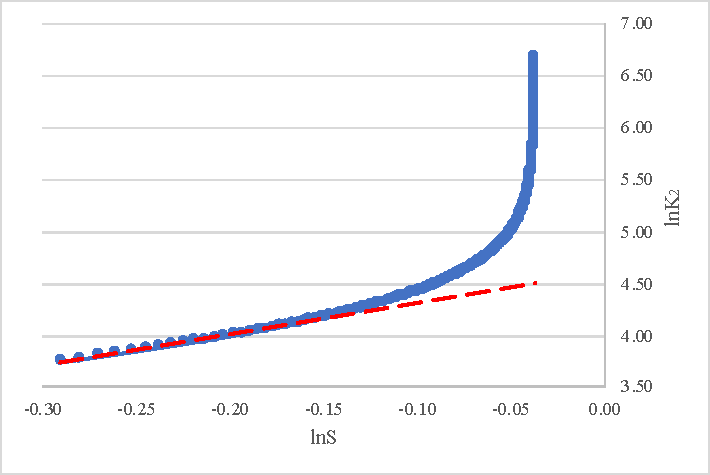
\includegraphics[width=0.8\linewidth]{1030.pdf} \\
	\caption[Scaling relation]{Scaling Relation}
	\label{fig:scaling}
\end{figure}
The slope is $3.02$, which implies $K_2^*\sim S^3$ at moderate nematic order.

\section{Comparison with Simulation Results}
Comparing with the simulation results in Sec. \ref{Sec:SimRes}, we can see if our theory gives a very close result with the simulations on the isotropic-nematic transition point.
\begin{table}[H]
	\caption{Comparison with Simulation}
	\label{tab:compsim}
	\centering
	\begin{tabular}{c|cc}
		\toprule
		Transition Point & Pressure $P_0^*$ & Packing Fraction $\eta_0$ \\
		\midrule
		Theory &  $1.451$ & $0.269$\\
		Simulation & $1.332$ & $0.240$\\
		\bottomrule
	\end{tabular}
\end{table}

From Tab. \ref{tab:compsim} we can see that both transition pressure and packing fraction are very close. The transition pressure and packing is a bit larger than that of the simulation. This is due to the assumption that the two-body radial distribution function to be $1$. If the correct RDF is calculated, particles that and lean on each other at a short distance and on a preferred angle will contribute more to the free energy calculation, which will lower the transition point. This is the motivation of our future work.






% 全文总结
% !TEX root = ../thesis.tex

\begin{summary}
这里是全文总结内容。

2015 年 2 月 28 日,中央在北京召开全国精神文明建设工作表彰暨学雷锋志愿服务大会,
公布全国文明城市(区)、文明村镇、文明单位名单。上海交通大学荣获全国文明单位称
号。

全国文明单位这一荣誉是对交大人始终高度重视文明文化工作的肯定,是对交大长期以来文
明创建工作成绩的褒奖。在学校党委、文明委的领导下,交大坚持将文明创建工作纳入学校
建设世界一流大学的工作中,全体师生医护员工群策群力、积极开拓,落实国家和上海市有
关文明创建的各项要求,以改革创新、科学发展为主线,以质量提升为目标,聚焦文明创建
工作出现的重点和难点,优化文明创建工作机制,传播学校良好形象,提升社会美誉度,显
著增强学校软实力。2007 至 2012 年间,上海交大连续三届荣获“上海市文明单位”称
号,成为创建全国文明单位的新起点。

上海交大自启动争创全国文明单位工作以来,凝魂聚气、改革创新,积极培育和践行社会主
义核心价值观。坚持统筹兼顾、多措并举,将争创全国文明单位与学校各项中心工作紧密结
合,着力构建学校文明创建新格局,不断提升师生医护员工文明素养,以“冲击世界一流大
学汇聚强大精神动力”为指导思想,以“聚焦改革、多元推进、以评促建、丰富内涵、彰显
特色”为工作原则,并由全体校领导群策领衔“党的建设深化、思想教育深入、办学成绩显
著、大学文化丰富、校园环境优化、社会责任担当”六大板块共 28 项重点突破工作,全面
展现近年来交大文明创建工作的全貌和成就。

进入新阶段,学校将继续开拓文明创建工作新格局,不断深化工作理念和工作实践,创新工
作载体、丰富活动内涵、凸显创建成效,积极服务于学校各项中心工作和改革发展的大局
面,在上级党委、文明委的关心下,在学校党委的直接领导下,与时俱进、开拓创新,为深
化内涵建设、加快建成世界一流大学、推动国家进步和社会发展而努力奋斗!

上海交通大学医学院附属仁济医院也获得全国文明单位称号。
\end{summary}


% 使用英文字母对附录编号
\appendix

% 附录内容,本科学位论文可以用翻译的文献替代。
%\input{tex/app_maxwell_equations}
%\input{tex/app_flow_chart}

% 文后无编号部分
\backmatter

% 参考资料
\printbibliography[heading=bibintoc]

% 用于盲审的论文需隐去致谢、发表论文、参与项目、申请专利、简历

% 致谢
% !TEX root = ../thesis.tex

%TC:ignore

\begin{acknowledgements}
	First of all, I am thankful for my parents, who gave me life and raised me up, and most importantly, they are always supporting me to find what I really need. I am also very grateful for my advisor Liang Wu and Huai Sun, they never ceases to encourage me, and helped me a lot in both study and life, Prof. Huai Sun treated me so kind and inspired me a lot to find what I yearn for. And I would like to thank the great teachers I met in Zhiyuan College these four years, Huai Sun and Liang Wu, who led me into this project, Cuipo Jiang, who taught me mathematics and gave me a first taste of modern mathematics, Xiangjun Xing, who gave an impressive lecture on statistical mechanics and enabled me to do hard derivations, Pu Zhang, who treated me so kind and encouragingly and helped a lot when I applied to graduate school. At last, I would thank my friends and classmates, who encouraged and trusted me in the past four years, thanks to Yu Zhou and Yanze Wu, they has guided me a lot when I applied to summer research program, thanks to my roommate Jie Xie, he has helped me a lot on computer technology, and thanks to Yang Zhang who has been my friend for seven years always inspired me when I am down, thanks to Runkang Feng who had helped a lot when I was a freshman in mathematics. I am grateful for been in Zhiyuan College, SJTU for four years, all my experience has made what I am today.
\end{acknowledgements}

%TC:endignore


% 发表论文、参与项目、申请专利、简历
% 盲审论文中,发表学术论文及参与科研情况等仅以第几作者注明即可,不要出现作者或他人姓名

%\input{tex/publications}
%\input{tex/projects}
%\input{tex/patents}
%% !TEX root = ../thesis.tex

%TC:ignore

\begin{resume}
  \subsection*{Fundamental Information}
    WEN, Cong, born on 12.01.1998

  \subsection*{教育背景}
  \begin{itemize}
    \item yyyy 年 mm 月至今,上海交通大学,博士研究生,xx 专业
    \item yyyy 年 mm 月至 yyyy 年 mm 月,上海交通大学,硕士研究生,xx 专业
    \item yyyy 年 mm 月至 yyyy 年 mm 月,上海交通大学,本科,xx 专业
  \end{itemize}

  \subsection*{联系方式}
  \begin{itemize}
    \item 地址: 上海市闵行区东川路 800 号,200240
    \item E-mail: \email{xxx@sjtu.edu.cn}
  \end{itemize}
\end{resume}

%TC:endignore


% 中文学士学位论文要求在最后有一个英文大摘要,单独编页码,英文学士学位论文不需要
%\input{tex/end_english_abstract}

\end{document}
